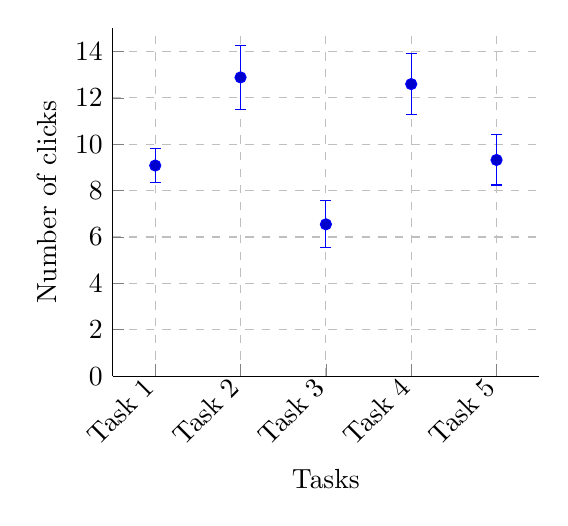
\begin{tikzpicture}[scale=1.0],
\centering
\begin{axis}[
height=6cm,
width=7cm, 
  xlabel={Tasks},
  ylabel={Number of clicks}, 
  ymax=15,
  ymin=0,
  xmin=0.5,
  xmax=5.5,
  axis y line*=left,
  axis x line*=bottom,
  xticklabels={Task 1,Task 2,Task 3,Task 4,Task 5},
  xtick={1,...,5},
  ytick={0,2,...,200},
        ymajorgrids=true,
      xmajorgrids=true,
      grid style=dashed,
  x tick label style={rotate=45,anchor=east}]
\addplot+[only marks][error bars/.cd,y dir=both, y explicit]
coordinates {
(1,9.08) +- (0.731,0.731)
(2,12.88) +- (1.3855,1.3855)
(3,6.5455) +- (1.0107,1.0107)
(4,12.591) +- (1.3126,1.3126)
(5,9.32) +- (1.0793,1.0793)
};
\addplot[dashed] coordinates {(0,0) (5.5,0)};
\end{axis}
\end{tikzpicture}%